\section{Calculus}

\formdesc{Tangent and Secant Lines}

\begin{itemize}
  \item Tangent line is the line on $f(x)$ at point $x = a$ that just touches the
	graph of the function
	    \begin{itemize}
	        \item The slope of a non-linear function at one point
	    \end{itemize} 
	    
	    \begin{center}
	        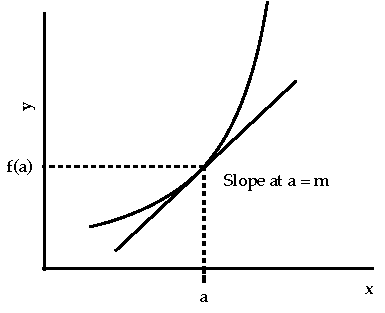
\includegraphics{tangent_line}
	    \end{center}
	    
  \item Secant line is the line between $A$ and $B$ on a curve
      \begin{center}
          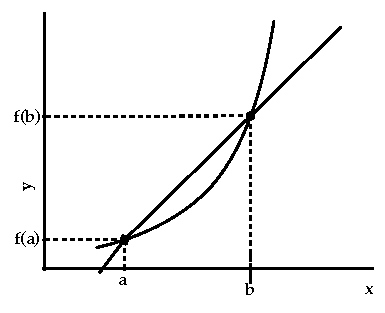
\includegraphics{secant_line}
      \end{center}
\end{itemize}

\textit{Note}: As $A$ gets	closer to $B$ the secant slope approaches the tangent line
\hformbar



\formdesc{Average Rate of Change}

\begin{equation}
    ARC = f(a, a + \Delta) = \frac{\Delta y}{\Delta x} = \frac{f(a + \Delta x) - f(a)}{\Delta x}
\end{equation}

over interval $[a, a + \Delta x]$
\hformbar



\formdesc{Derivative}

The instantaneous rate of change of a function $f(x)$ at point $x = a$

\begin{equation}
    f'(a) = \lim_{\Delta x \to 0} \frac{\Delta y}{\Delta x} = \lim_{\Delta x \to 0} \frac{f(a + \Delta x) - f(a)}{\Delta x}
\end{equation}

``the derivative of $y$ w.r.t. $x$'' $\equiv \frac{dy}{dx} \equiv \lim_{\delta \rightarrow 0} \frac{\delta y}{\delta x}$

\hformbar







\formdesc{Simple Derivatives}

\begin{center}
\[
\def\arraystretch{2.5}
 \begin{array}{cc}
  \textit{y}   &      \textit{y'}             \\
  \midrule
  k            & 0                             \\
  x            & 1                             \\ 
  x^n          & nx^{n-1}                      \\
  \sqrt{x}     & \dfrac{1}{2\sqrt{x}}          \\
  \sqrt[n]{x}  & \dfrac{1}{n\sqrt[n]{x^{n-1}}} \\
  \dfrac{1}{x} & \dfrac{-1}{x^2}               \\ 
  e^x          & e^x                           \\
  a^x          & a^x\ln(a)                     \\
  x^x          & xx^{x-1}+x^x\ln(x)            \\
  \ln(x)       & \dfrac{1}{x}                  \\
  \log_a(x)    & \dfrac{1}{x}\log_a(e)         
 \end{array}
\]
\end{center}
\hformbar



\formdesc{Composite Derivatives}

\begin{center}
\[
\def\arraystretch{2.5}
 \begin{array}{cc}
  \textit{y}   &      \textit{y'}               \\
  \midrule
  u^n          & nu^{n-1}u'                     \\
  \sqrt{u}     & \dfrac{u'}{2\sqrt{u}}          \\
  \sqrt[n]{u}  & \dfrac{u'}{n\sqrt[n]{u^{n-1}}} \\
  \dfrac{1}{u} & \dfrac{-u'}{u^2}               \\
  e^u          & e^u u'                         \\
  a^u          & a^u\ln(a)u'                    \\
  u^v          & vu^{v-1}u'+u^v\ln(u) v'        \\
  \ln(u)        & \dfrac{u'}{u}                 \\
  \log_a(u)    & \dfrac{u'}{u}\log_a(e)
 \end{array}
\]
\end{center}
\hformbar



\formdesc{Derivative Operations}

\begin{center}
  \begin{tabular}{ll}
  Sum         & $(f(x)+g(x))' = f'(x) + g'(x)$    \\
  Difference  & $(f-g)'(x) = f'(x) - g'(x)$        \\
  Product     & $(fg)'(x) = f'(x)g(x) + f(x)g'(x)$ \\
  Quotient    & $ \left(\frac{f(x)}{g(x)}\right)' = \frac{f'(x)g(x) - f(x)g'(x)}{g(x)^2}$ \\
  Chain rule  & $(f(g))'(x) = f'(g(x))g'(x)$        \\
  Inverse     & $(f^{-1})'(x) = \frac{1}{f'(x)}$  
  \end{tabular}
\end{center}
\hformbar






\formdesc{Limits}

\begin{equation}
    \lim_{x \rightarrow C} f(x) = L
\end{equation}

or, ``the limit of $f(x)$, as $x$ approaches $c$, is $L$.'' $\lim_{x \rightarrow C} f(x)$ is a \textit{single number} that describes the behavior of the function $f(x)$ \textit{near} but not \textit{at} the point $x = c$.

Introduced to make calculating rate of change at 0 feasible, by making the $\Delta$ so infinitesimal the difference is between it and 0 is negligible---``allows'' division by 0

\subsection*{Example}

\begin{center}
    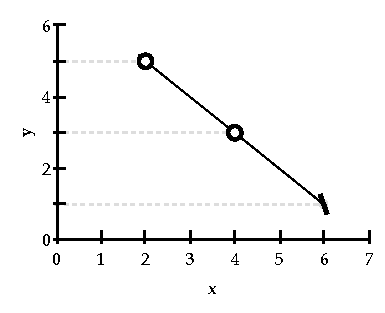
\includegraphics{linear_limits2}
\end{center}

where hollow points are undefined and solid points are defined

\begin{enumerate}
    \item $\lim_{x \rightarrow 6} f(x) = 1$
    \item $\lim_{x \rightarrow 4} f(x) = 3$
        \begin{itemize}
            \item \textit{Note}: even though $x=4$ is undefined, we're only concerned with the area \textit{around} 4, so we can still find the limit
        \end{itemize}
    \item $\lim_{x \rightarrow 2} f(x) = 5$
\end{enumerate}

\subsection*{Example: Determining Limits of Non-Linear Functions}

\begin{center}
    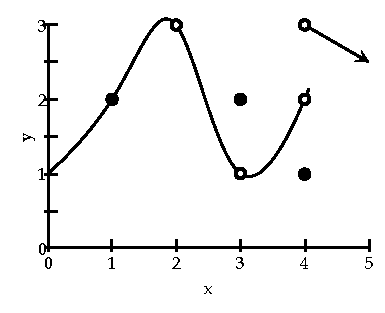
\includegraphics{limits_ex2}
\end{center}

where hollow points are undefined and solid points are defined

\begin{enumerate}
    \item $\lim_{x \rightarrow 1} f(x) = 2$---values where $x$ is close to but not equal to 1 are near 2
    \item $\lim_{x \rightarrow 2} f(x) = 3$---even though $f(2)$ is undefined, only values \textit{near} $f(2)$ are important
    \item $\lim_{x \rightarrow 3} f(x) = 1$---even though $f(3)$ is actually 2
    \item $\lim_{x \rightarrow 4} f(x) =$ \textit{does not exist}: Can't determine a single number because $f(4)$ from the right is about 2, and from the left about 3
\end{enumerate}


\subsection*{Example: Determining Limits Using Algebra}

Factor equation to simplest form and plug in $c$ (assuming function at $c$ is defined):

\begin{equation}
    \lim_{x \rightarrow 5} \frac{x^2 - 6x + 8}{x - 4} = \frac{25 - 30 + 8}{1} = 3
\end{equation}
\hformbar



\formdesc{Limits of Broken Functions}

Some functions are continuous but in an unusual way---they appear ``broken'' when graphed---and so there is a \textit{left} and \textit{right} limit

\begin{description}
    \item[Left] ``The limit coming from the left''; values of $f(x)$ as $f(x)$ nears $x$ and left of $c$, $x < c$
        \begin{equation}
            \lim_{x \rightarrow c^-} f(x) = L
        \end{equation}
    \item[Right] ``This limit coming from the right''; values of $f(x)$ as $f(x)$ nears $x$ and right of $c$, $x > c$
        \begin{equation}
            \lim_{x \rightarrow c^+} f(x) = L
        \end{equation}
    
\end{description}

\textit{Note}: If left and rights limits are not the same, limit \textit{doesn't exist}.
\hformbar



\formdesc{Continuity}

A function $f$ is continuous at $x = a$ iff $\lim_{x \rightarrow a} f(x) = f(a)$,
i.e., if the limit of $x$ at $a$ is equals $f(a)$, i.e., no breaks or jumps

\subsection*{Example}

\begin{center}
    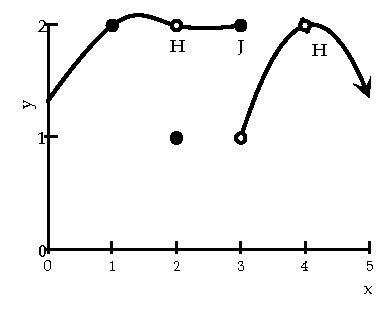
\includegraphics{continuity}
\end{center}

where $H$ indicates a hole---where the graph is defined but could be made continuous by changing the point---and $J$ a jump---where the left and right limits are not the same.

\begin{itemize}
    \item Continuous at 1 since $\lim_{x \rightarrow 1} f(x) = f(1) = 2$
    \item Not continuous at 2, 3, or 4
        \begin{itemize}
            \item $\lim_{x \rightarrow 2} f(x) =2 \neq f(2) = 1$
            \item $\lim_{x \rightarrow 3} f(x) =$ doesn't exist $\neq f(3) = 2$
            \item $\lim_{x \rightarrow 4} f(x) = 2 \neq f(4) =$ undefined
        \end{itemize}

\end{itemize}
\hformbar



\formdesc{Calculating Derivatives}

\subsection*{Example: Using Formal Definition}

Find derivative of $f(x) = 2x^2 - 16x + 35$.

\begin{enumerate}
    \item Assemble using the formal definition
        \begin{equation}
            \frac{\left[ 2(x - h)^2 - 16(x + h) + 35 \right] - 
                \left[ 2x^2 - 16x - 35 \right] }{h}
        \end{equation}
        
    \item Factor---\textit{cannot plug $h=0$ because no division by zero!}
        \begin{eqnarray}
            &=& \frac{2x^2 + 4xh + 2h^2 - 16x - 16h + 35 - 2x^2 + 16x - 35}{h} \\
            &=& \lim_{h \rightarrow 0} \frac{4xh + 2h^2 - 16h}{h}
        \end{eqnarray}
        
    \item Factor out $h$ in numerator to cancel $h$ in denominator
        \begin{eqnarray}
            f'(x) &=& \lim_{h \rightarrow 0} \frac{h(4x + 2h - 16)}{h} \\
            &=& \lim_{h \rightarrow 0} 4x + 2h - 16 \\
            &=& 4x - 16
        \end{eqnarray}

\end{enumerate}
\hformbar



\formdesc{Implicit Differentiation}

The process to find $y' = f'(x)$ when $f(x)$ is difficult or impossible to use with explicit differentiation, by assuming $y$ is a function of $x$:

\subsection*{Example}

Implicitly differentiate $x^2 + y^2 = 25$

\begin{enumerate}
    \item Differentiate each side, treating $y$ as a function
    \begin{eqnarray}
        \frac{d}{dx} \left( x^2 + y^2 \right) = \frac{d}{dx} 25 \\
        &\Rightarrow& \frac{d}{dx} x^2 + \frac{d}{dx} y^2 = 0 \\
        &\Rightarrow& 2x + 2y \frac{dy}{dx} = 0 \\
        &\Rightarrow& 2x + 2yy' = 0
    \end{eqnarray}
    
    \item Algebraically solve for $y'$
    \begin{eqnarray}
    	2yy' = -2x \\
	    &\Rightarrow& y' = \frac{-2x}{2y} \\
	    &\Rightarrow& y' = -\frac{x}{y}    
    \end{eqnarray}
\end{enumerate}
\hformbar



\formdesc{Definite Integral}

The definite integral of a positive function $f(x)$ over an interval $[a, b]$ is the area between $f$, the $x$-axis, $x = a$, and $x = b$.

\begin{equation}
    \int_a^b f(x)\, dx
\end{equation}

where $a$ and $b$ are the ``limits of integration'' and $f(x)$ is the integrand

    \begin{eqnarray}
        \int_a^a f(x)\, dx &=& 0                   \\
        \int_a^b f(x)\, dx &=& -\int_b^a f(x)\, dx  \\
        \int_a^b f(x)\, dx &=& \int_a^c f(x)\, dx + \int_c^b f(x)\, dx
    \end{eqnarray}

where $a<c<b$
\hformbar



\formdesc{Integration Operations}

\begin{center}
  \begin{tabular}{ll}
  Sum           & $\int u+v\,dx = \int u\,dx + \int v\,dx$  \\
  Difference    & $\int u-v\,dx = \int u\,dx - \int v\,dx$  \\
  Product       & $\int af(x)\,dx = a\int f(x)\,dx$         \\
  Parts         & $\int u\,dv = uv - \int v\,du$            \\
  Substitution  & $\int f(u)u'\,dx = \int f(u)\,du$
  \end{tabular}
\end{center}
\hformbar



\formdesc{Growth, Concavity, and Extrema}

\flushleft
			\begin{description}
				\item[Growth]
				      \begin{itemize}
					      \item[]
					      \item $\forall x\in I\ f'(x)\geq 0$ $\Rightarrow$ $f$ is increasing in $I$.
					      \item $\forall x\in I\ f'(x)\leq 0$ $\Rightarrow$ $f$ is decreasing in $I$.
				      \end{itemize}
				\item[Concavity]
				      \begin{itemize}
					      \item[]
					      \item $\forall x\in I\ f''(x)\geq 0$ $\Rightarrow$ $f$ is concave up in $I$.
					      \item $\forall x\in I\ f''(x)\leq 0$ $\Rightarrow$ $f$ is concave down in $I$.
				      \end{itemize}
				\item[Extrema] If $f'(a)=0$ (critical point)
				      \begin{itemize}
					      \item $f''(a)<0$ $\Rightarrow$ $f$ has a local maximum at $x=a$.
					      \item $f''(a)>0$ $\Rightarrow$ $f$ has a local minimum at $x=a$.
				      \end{itemize}
			\end{description}

\begin{figure}[h]
\centering
\begin{minipage}{.5\linewidth}
  \centering
  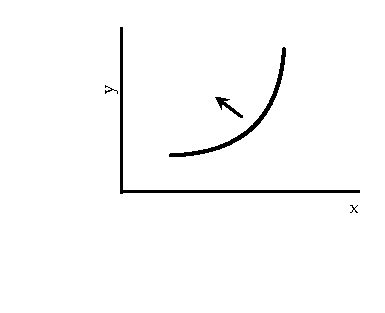
\includegraphics[trim={0 45pt 0 0},clip,width=.8\linewidth]{concave_up}
\end{minipage}%
\begin{minipage}{.5\linewidth}
  \centering
  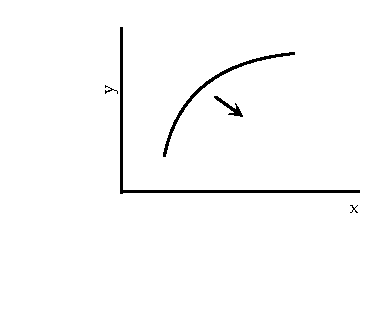
\includegraphics[trim={0 45pt 0 0},clip,width=.8\linewidth]{concave_down}
\end{minipage}
\caption{Concave up (left) and concave down (right)}
\end{figure}
\hformbar



\formdesc{Increasing and Decreasing Functions}

\begin{itemize}
    \item $f(x)$ is \textit{increasing} iff $\forall~ x_1, x_2$ in interval $I$ is such that $x_1 < x_2$ and $f(x_1) < f(x_2)$
    \item $f(x)$ is \textit{decreasing} iff $\forall~ x_1, x_2$ in interval $I$ is such that $x_1 > x_2$ and $f(x_1) > f(x_2)$
    \item Determine all intervals where $f(x)$ is in/decreasing:
    \begin{enumerate}
        \item Find all critical points (via first deriative)
        \item For each critical point, select a number $a$ in that range and see if $f'(a)$ is positive or negative
    \end{enumerate}
\end{itemize}


\hformbar



\formdesc{Inflection Points}

\begin{itemize}
    \item Where the second derivative changes signs
    \item The point(s) on a graph where the concavity of a function changes from up to down
    \item functions can be increasing (positive derivative) or decreasing (negative derivative) regardless of concavity,
\end{itemize}
\hformbar






\formdesc{Maxima And Minima}

A \textit{critical point} is a point where either $f'(a) = 0$ or $f'(a)$ is undefined, and is a \textit{candidate} of being a local or global extreme

\subsection*{Local}

\begin{description}
    \item[maximum] at $a$ if $f(a) \geq f(x)~ \forall x$ near $a$
    \item[minimum] at $a$ if $f(a) \leq f(x)~ \forall x$ near $a$
    \item[extreme] at $a$ if $f(a)$ is a local maximum or minimum
\end{description}
    
\subsection*{Global}

\begin{description}
    \item[maximum] at $a$ if $f(a) \geq f(x)~ \forall x$ in domain of $f$
    \item[minimum] at $a$ if $f(a) \leq f(x)~ \forall x$ in domain of $f$
    \item[extreme] at $a$ if $f(a)$ is a global maximum or minimum
\end{description}

\subsection*{Example}

Find the critical point of $f(x) = x^3 - 6x^2 + 9x + 2$

\begin{enumerate}
    \item Find $f'(x)$
        \begin{eqnarray}
            f'(x)  =  3x^2 - 12x + 9  \\
                  &=& 3(x^2 - 4x + 3) \\
                  &=& 3(x - 1)(x - 3) \\
         \end{eqnarray}
     \item Find where $f'(x) = 0$, which is 1 and 3
     \item Put $x=1$ and $x=3$ into $f(x)$ to find the critical points
         \begin{eqnarray}
             (1, f(1)) &=& (1, 6) \\
             (3, f(2)) &=& (3, 2)         
         \end{eqnarray}
\end{enumerate}
\hformbar



\formdesc{Antiderivatives}

\begin{itemize}
    \item \textit{An} antiderivative of a function $f(x)$ is any function $F(x)$ such that $F'(x) = f(x)$
    \item \textit{The} antiderivative is an entire family of functions, written $F(x) + c$
    \item Also known as the \textit{indefinite integral} (with no limit markers):
    
    \begin{equation}
        \int f(x)~ dx
    \end{equation}
\end{itemize}

\subsection*{Example}

\textit{An} antiderivative of $\int 2x~ dx$ is $x^2 - 5.2$; \textit{the} antiderative is $x^2 + C$
\hformbar



\formdesc{Definite v. Indefinite Integrals}

Indefinite integrals do not have limits to integration where definite integrals do
\hformbar



\formdesc{Integration by Substitution}

A method to algebraically manipulate an integrand so it is amenable to antiderivative rules; especially useful when there is a product in the integral.

Substitute $u$ for $g(x)$ where necessary, making $\frac{du}{dx} = g'(x)$, so $du = g'(x)~ dx$. Since

\begin{equation}
    \frac{du}{dx} = g'(x) \equiv du = g'(x)~ dx
\end{equation}

we can substitute so that

\begin{equation}
    \int f'(g(x)) g'(x)~ dx \equiv \int f'(u)~ du
\end{equation}

Now integrate $f'(u)~ du$. (Note that $g(x) \equiv u$ and $g'(x)~ dx \equiv du$.)

\begin{enumerate}
    \item Set one part of the integrand to $u$, one ``level'' into the integral
    \item Compute $du = \frac{du}{dx} ~dx$ (the derivative of $u$)
    \item Convert $x$'s to $u$'s in original integral, even including in $dx$
    \item Integrate new $u$ integral
    \item Substitute $u$'s back to $x$'s in integral
\end{enumerate}

\subsection*{Example}

Integrate $\int (x + 1)^3~ dx$

\begin{enumerate}
	\item Rearrange so that $u = x + 1$ and $du = 1~ dx$
		\begin{equation}
			= \int (x + 1)^3 \cdot 1 ~ dx
		\end{equation}
	\item Substitute in $u$ and $du$
		\begin{equation}
			\int u^3 ~ du
		\end{equation}
	\item Integrate
		\begin{equation}
			= \frac{u^4}{4} + C
		\end{equation}
	\item Add $u$ back in
		\begin{equation}
			= \frac{(x + 1)^4}{4} + C
		\end{equation}
\end{enumerate}

\hformbar



\formdesc{Integration by Parts}

Integrate a complex function by rewriting it as a product of two simpler functions $u$ and $du$, using two possible forms:

\begin{eqnarray}
  \int u ~dv     &=& uv - \int v ~du \\
  \int_a^b u ~dv &=& uv |_a^b - \int_a^b v ~du
\end{eqnarray}

\subsection{Example: First Form}

Integrate $\int xe^x ~dx$:

\begin{enumerate}
  \item Break into two parts: $u = x$ and $dv = e^x ~dx$
  \item Calculate the derivative of $u$, $~du$, and $v$, the integral of $dv$
	\begin{eqnarray}
	  du &=& \left( \frac{d}{dx} x \right) ~dx = 1 ~dx \\
	  v &=& \int dv = \int e^x ~dx = e^x
	\end{eqnarray}
  \item Using the first formula, noting the prior forms from 1 and 2
	\begin{eqnarray}
      \int u ~dv &=& \int x e^x ~dx \\
	             &=& xe^x - \int e^x ~dv \\
				 &=& xe^x - e^x + C
     \end{eqnarray}
\end{enumerate}

\subsection{Example: Second Form}

Integrate $\int_1^4 6x^2 ln x ~dx$:

\begin{enumerate}
	\item Break into two parts: $u = ln x$ and $dv = 6x^2$
	\item Calculate the derivative of $u$, $du$, and the integral of $dv$, $v$:
	  \begin{eqnarray}
	    du &=& \frac{d}{dx} ln x = \frac{1}{x} ~dx \\
		v  &=& \int 6x^2 ~dx = 6 \int x^2 ~dx = 6 \cdot \frac{x^3}{3} = 2x^3
	  \end{eqnarray}
	\item Use the second formula
	  \begin{eqnarray}
	    \int_1^4 6x^2 ln x ~dx &=& 2x^3 ln x |_1^4 - \int_1^4 2x^3 \frac{1}{x} ~dx \\
		&=& 2x^3 ln x |_1^4 - 3x^2 |_1^4
	  \end{eqnarray}
	\item Find the integral the usual way:
	  \begin{eqnarray}
	    \left[ (2 \cdot 4^3 ln(4)) - (2 \cdot 1^3 ln(1)\right] - \left[ (3 \cdot 4^2) - (3 \cdot 1^2)  \right] \\
		  = 128 \cdot ln(4) - 45 \\
		  \approx 132.446
	  \end{eqnarray}
\end{enumerate}





\hformbar












\formdesc{Antiderivative Rules}

\begin{center}
\[
\def\arraystretch{2.5}
 \begin{array}{cc}
  \int a\,dx              & ax+C                   \\
  \int x^n\,dx            & \dfrac{u'}{2\sqrt{u}}  \\
  \int e^x\,dx            & e^x+C                  \\
  \int a^x\,dx           & \dfrac{a^x}{\ln(a)}+C  \\
  \int \dfrac{1}{x}\, dx  &  \ln|x|+C
 \end{array}
\]
\end{center}
\hformbar










\newpage
